\let\negmedspace\undefined
\let\negthickspace\undefined
\documentclass[journal,12pt,twocolumn]{IEEEtran}

\usepackage{cite}
\usepackage{amsmath,amssymb,amsfonts,amsthm}
\usepackage{algorithmic}
\usepackage{graphicx}
\usepackage{textcomp}
\usepackage{xcolor}
\usepackage{txfonts}
\usepackage{listings}
\usepackage{enumitem}
\usepackage{mathtools}
\usepackage{gensymb}
\usepackage[breaklinks=true]{hyperref}
\usepackage{tkz-euclide} % loads  TikZ and tkz-base
\usepackage{listings}
\usepackage{circuitikz}
\usepackage{graphicx}

%\newcounter{MYtempeqncnt}
\DeclareMathOperator*{\Res}{Res}
%\renewcommand{\baselinestretch}{2}
\renewcommand\thesection{\arabic{section}}
\renewcommand\thesubsection{\thesection.\arabic{subsection}}
\renewcommand\thesubsubsection{\thesubsection.\arabic{subsubsection}}

\renewcommand\thesectiondis{\arabic{section}}
\renewcommand\thesubsectiondis{\thesectiondis.\arabic{subsection}}
\renewcommand\thesubsubsectiondis{\thesubsectiondis.\arabic{subsubsection}}

% correct bad hyphenation here
\hyphenation{op-tical net-works semi-conduc-tor}
\def\inputGnumericTable{}                                 %%

\lstset{
	frame=single,
	breaklines=true,
	columns=fullflexible
}



\newtheorem{theorem}{Theorem}[section]
\newtheorem{problem}{Problem}
\newtheorem{proposition}{Proposition}[section]
\newtheorem{lemma}{Lemma}[section]
\newtheorem{corollary}[theorem]{Corollary}
\newtheorem{example}{Example}[section]
\newtheorem{definition}[problem]{Definition}
\newcommand{\BEQA}{\begin{eqnarray}}
	\newcommand{\EEQA}{\end{eqnarray}}
\newcommand{\define}{\stackrel{\triangle}{=}}
\newcommand\figref{Fig.~\ref}
\newcommand\tabref{Table~\ref}
\bibliographystyle{IEEEtran}
%\bibliographystyle{ieeetr}


\providecommand{\mbf}{\mathbf}
\providecommand{\pr}[1]{\ensuremath{\Pr\left(#1\right)}}
\providecommand{\qfunc}[1]{\ensuremath{Q\left(#1\right)}}
\providecommand{\sbrak}[1]{\ensuremath{{}\left[#1\right]}}
\providecommand{\lsbrak}[1]{\ensuremath{{}\left[#1\right.}}
\providecommand{\rsbrak}[1]{\ensuremath{{}\left.#1\right]}}
\providecommand{\brak}[1]{\ensuremath{\left(#1\right)}}
\providecommand{\lbrak}[1]{\ensuremath{\left(#1\right.}}
\providecommand{\rbrak}[1]{\ensuremath{\left.#1\right)}}
\providecommand{\cbrak}[1]{\ensuremath{\left\{#1\right\}}}
\providecommand{\lcbrak}[1]{\ensuremath{\left\{#1\right.}}
\providecommand{\rcbrak}[1]{\ensuremath{\left.#1\right\}}}
\theoremstyle{remark}
\newtheorem{rem}{Remark}
\newcommand{\sgn}{\mathop{\mathrm{sgn}}}
\providecommand{\abs}[1]{\left\vert#1\right\vert}
\providecommand{\res}[1]{\Res\displaylimits_{#1}}
\providecommand{\norm}[1]{\left\lVert#1\right\rVert}
%\providecommand{\norm}[1]{\lVert#1\rVert}
\providecommand{\mtx}[1]{\mathbf{#1}}
\providecommand{\mean}[1]{E\left[ #1 \right]}
\providecommand{\fourier}{\overset{\mathcal{F}}{ \rightleftharpoons}}
%\providecommand{\hilbert}{\overset{\mathcal{H}}{ \rightleftharpoons}}
\providecommand{\system}{\overset{\mathcal{H}}{ \longleftrightarrow}}
%\newcommand{\solution}[2]{\textbf{Solution:}{#1}}
\newcommand{\solution}{\noindent \textbf{Solution: }}
\newcommand{\cosec}{\,\text{cosec}\,}
\providecommand{\dec}[2]{\ensuremath{\overset{#1}{\underset{#2}{\gtrless}}}}
\newcommand{\myvec}[1]{\ensuremath{\begin{pmatrix}#1\end{pmatrix}}}
\newcommand{\mydet}[1]{\ensuremath{\begin{vmatrix}#1\end{vmatrix}}}
\renewcommand{\abstractname}{Question}

\let\vec\mathbf

	
	\vspace{3cm}
	
	


\newcommand{\permcomb}[4][0mu]{{{}^{#3}\mkern#1#2_{#4}}}
\newcommand{\comb}[1][-1mu]{\permcomb[#1]{C}}

%\IEEEpeerreviewmaketitle

\newcommand \tab [1][1cm]{\hspace*{#1}}
%\newcommand{\Var}{$\sigma ^2$}
\usepackage{amssymb}
\usepackage{amsmath}
\title{
	
\title{NCERT Physics 11.15 Q14}
\author{EE23BTECH11212 - ABBURI TANUSHA$^{*}$% <-this % stops a space
}


}
\begin{document}

\maketitle

\textbf{Question:} 
A wire stretched between two rigid supports vibrates in its fundamental mode with a frequency of $45 \, \text{Hz}$. The mass of the wire is $3.5 \times 10^{-2} \, \text{kg}$, and its linear mass density is $4 \times 10^{-2} \, \text{kg/m}$. The length of the wire is $0.875 \, \text{m}$. Determine the speed of a transverse wave on the string and the tension in the string.
\\
     
\textbf{Solution: }
The following information is provided in the question:

 \begin{table}[h]
 	\centering
 	\resizebox{6 cm}{!}{
 		

    \begin{tabular}{|c|c|c|}
        \hline
        \textbf{Parameter} & \textbf{Value} & \textbf{Description} \\
        \hline
        a     & 8 & First term \\
        d     & 5 & common difference\\
        xi(0) & 8 & First term \\
        \hline
    \end{tabular}
    
    



 	}
 	\vspace{6 pt}
 	\caption{Parameters}
 	\label{tab:my_label} 
 \end{table}
 
 To derive the expression for the speed of a transverse wave on a stretched string, let's start with Newton's second law applied to a small segment of the string. Consider a small element of the string of length $\Delta x$ and mass $\Delta m$. The tension force $T$ is acting in the positive $y$-direction, and the displacement of the string is in the $y$-direction.
 
\begin{figure}[h]
	\centering
	

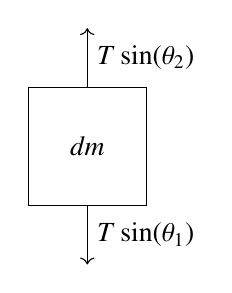
\begin{tikzpicture}[scale=0.75] % Adjust the scale factor as needed
    % Draw the square body
    \draw (0,0) rectangle node[pos=0.5] {$dm$} (2,2);
    
    % Add upward force T*sin(theta2)
    \draw[->, black] (1,2) -- node[right] {$T \sin(\theta_2)$} (1,3);
    
    % Add downward force T*sin(theta1)
    \draw[->, black] (1,0) -- node[right] {$T \sin(\theta_1)$} (1,-1);
\end{tikzpicture}




	\caption{FBD OF THE BODY}
	\label{fig:2}
\end{figure}

From the figure~\figref{fig:2} the net force in the $y$-direction is given by 
\begin{equation}\label{eq:force}
    F_y = T \sin(\theta) - (T + \Delta T) \sin(\theta + \Delta \theta),
\end{equation}
where $\theta$ is the angle of displacement.

Applying Newton's second law $F = ma$ to this element in the $y$-direction:
\begin{equation}\label{eq:newton}
    \Delta m \frac{\partial^2y}{\partial t^2} = T \sin(\theta) - (T + \Delta T) \sin(\theta + \Delta \theta).
\end{equation}

For small angles $\theta$, $\sin(\theta) \approx \theta$, and we can simplify the expression:
\begin{equation}\label{eq:simplified}
    \Delta m \frac{\partial^2y}{\partial t^2} = T \theta - (T + \Delta T)(\theta + \Delta \theta).
\end{equation}

Rearrange and divide by $\Delta x$ to get the linear density $\mu$:
\begin{equation}\label{eq:linear_density}
    \frac{\partial^2y}{\partial t^2} = \frac{T}{\mu} \theta - \frac{T}{\mu} \frac{\Delta T}{T}(\theta + \Delta \theta).
\end{equation}

Now, take the limit as $\Delta x$ approaches zero and replace $\theta$ with $\frac{\partial y}{\partial x}$:
\begin{equation}\label{eq:limit}
    \frac{\partial^2y}{\partial t^2} = \frac{T}{\mu} \frac{\partial y}{\partial x} - \frac{T}{\mu} \frac{\partial}{\partial x} \left(\frac{\Delta T}{T}\frac{\partial y}{\partial x}\right).
\end{equation}

Now, assume that the displacement is a sinusoidal wave of the form $y(x, t) = A \sin(kx - \omega t)$. Substitute this into the equation and solve for $v$:
\begin{equation}\label{eq:wave_speed}
    v = \sqrt{\frac{T}{\mu}}.
\end{equation}

This completes the derivation of the wave speed using first principles.

\textbf{1. Find the wavelength (\(\lambda\)) for the fundamental mode:}
\begin{equation}\label{eq:wavelength}
    \lambda = 2L \quad \Rightarrow \quad \lambda = 2 \times 0.875 \, \text{m} = 1.75 \, \text{m}
\end{equation}

\textbf{2. Use the frequency and wavelength to find the wave speed (\(v\)):}
\begin{equation}\label{eq:wavespeed}
    v = f \cdot \lambda \quad \Rightarrow \quad v = 45 \, \text{Hz} \times 1.75 \, \text{m} = 78.75 \, \text{m/s}
\end{equation}


\textbf{3. Use the wave speed (\(v\)) to find the tension (\(T\)) using the wave equation:}
\begin{equation}\label{eq:tension}
    T = \mu \cdot v^2 \quad \Rightarrow \quad T = (4 \times 10^{-2} \, \text{kg/m}) \times (78.75 \, \text{m/s})^2 = 123.1875 \, \text{N}
\end{equation}

Therefore, the speed of the transverse wave on the string is $78.75 \, \text{m/s}$, and the tension in the string is $123.1875 \, \text{N}$.

\end{document}
